\documentclass[a4paper,portrait]{scrartcl}
\author{Andreas Mai}
\title{HM I + II Zusammenfassung KIT}
\usepackage[utf8]{inputenc}
\usepackage[T1]{fontenc}
\usepackage{lmodern}
\usepackage[german]{babel}
\usepackage{graphicx}
\usepackage{amsmath}
\usepackage{mathtools}
\usepackage{amsfonts}
\usepackage{color}
\everymath{\displaystyle}
\begin{document}

\maketitle
\begin{center}
\textbf{HM Klausur am 30.08.2016} \\
\textbf{08:00 - 10:00 HM I} \\
\textbf{11:00 - 13:00 HM II} 
\end{center}

\begin{center}
\textit{Kein Anspruch auf Vollständigkeit ;)}
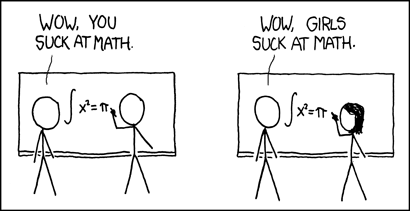
\includegraphics{how_it_works.png}

\end{center}
\clearpage
\tableofcontents
\clearpage
\setcounter{page}{1}
\section{Folgen und Reihen}
\subsection{Allgemein}
\begin{itemize}
	\item Eine Folge ist eine durchnummerierte Menge von Zahlen.  $(s_n)_{n \in \mathbb{N}}, s\in\mathbb{R}$
	\item Eine Reihe ist die Summe einer Folge.  $(s_m)_{m \in \mathbb{N}}, s\in\mathbb{R}$ \\ Eine Reihe ist auch eine Folge! $\sum_{i=1/0}^{n}(s_i),  s\in\mathbb{R}$
	\item Kleinste obere Schranke = Supremum
	\\Größte untere Schranke = Infimum
	\item Geometrische Reihe: $\sum_{i=0}^{n}q^i = \frac{q^{n+1} - 1}{q-1}, q \neq 1$
\end{itemize}
\subsection{Monotonie}
Zu faul, evtl später: https://youtu.be/Ii0b3L5UWZw

\subsection{Konvergenz}
\begin{itemize}
	\item Eine Folge (oder Reihe) ist konvergent, wenn sie gegen einen bestimmten Wert konvergiert.
	\item Sie ist bestimmt divergent, wenn sie gegen $ \pm  \infty $ läuft
	\item Sie ist unbestimmt divergent, wenn sich keine Aussage machen lässt \\ (bsp: 1 und -1 abwechseln).
	\item Formel: $\forall \varepsilon > 0: \exists n_0: \forall n \geq n_0: |s_n - g| < \varepsilon$ ($g$: Grenze)
\end{itemize}
\subsubsection*{Grenzwert bestimmen}
Grad der Funktion:
\begin{itemize}
  \item $Zählergrad < Nennergrad \Rightarrow  s_{n} \rightarrow 0$ \\
  Beispiel: $s_{n} = \frac{n}{n^2+4} \Rightarrow s_{n} \rightarrow 0$
  \item $Zählergrad = Nennergrad \Rightarrow  s_{n} \rightarrow Bruch$ \\
    Beispiel: $s_{n} = \frac{3n+4}{5n+96} \Rightarrow s_{n} \rightarrow \frac{3}{5}$
  \item $Zählergrad > Nennergrad \Rightarrow  s_{n} \rightarrow \infty \Rightarrow $ bestimmt divergent \\
    Beispiel: $s_{n} = \frac{n^6-7}{n^2+4} \Rightarrow s_{n} \rightarrow \infty$
\end{itemize}
\subsubsection*{Grenzwert beweisen}
Durch Formel.
\subsubsection*{Beispiel}
$ s_n = \frac{1}{n} $ \\
Zählergrad < Nennergrad $\Rightarrow  s_{n} \rightarrow 0$ \\
$ |s_n - g| = |\frac{1}{n} - 0| = \frac{1}{n} < \frac{1}{n_0} \leq \varepsilon$ \\
Drüber schreiben: Es sei $n_0 > \frac{1}{\varepsilon}$
\subsubsection{Nullfolgenkriterium}
$ \lim\limits_{n \rightarrow \infty} \neq 0 \Rightarrow \sum_{i=0}^{\infty} $ divergent \\
Die Folge der Reihe muss gegen 0 laufen, dass die Reihe konvergent sein kann (nicht umgekehrt!)
\subsubsection{Minorantenkriterium}
2 Reihen bekannt: $\sum_{n=0}^{\infty} s_n$ und $\sum_{n=0}^{\infty} t_n$ und zweitere divergiert (bestimmt). \\
Wenn für fast alle $n$ gilt: $ s_n \geq t_n \Rightarrow \sum_{n=0}^{\infty} s_n $ divergiert auch (bestimmt)
\subsubsection{Majorantenkriterium}
2 Reihen bekannt: $\sum_{n=0}^{\infty} s_n$ und $\sum_{n=0}^{\infty} t_n$ und zweitere konvergent \\
Wenn für fast alle $n$ gilt: $ |s_n| \leq t_n \Rightarrow \sum_{n=0}^{\infty} s_n $ absolut konvergent, umkehrung gilt nicht!
\subsubsection{Cauchykriterium}
$ \forall \varepsilon > 0 \exists n_0 \forall n,m \geq n_0: |\sum_{i=0}^{n} s_i - \sum_{i=0}^{m} s_i| = |\sum_{i=n}^{m} s_i| < \varepsilon$ \\
Wenn Cauchy-Kriterium erfüllt, konvergent ansonsten divergent
\subsubsection{Leibnitzkriterium}
\begin{itemize}
	\item $ \sum_{n=0}^{\infty} (-1)^n f_n $ mit $ \lim\limits_{n \rightarrow \infty} = 0,
	\begin{array}{ll}
	s_n \geq 0 \text{ monoton fallend } \\
	s_n \leq 0 \text{ monoton steigend } 
	\end{array}
	$ 
	\item Wenn Leibnitzkriterium erfüllt, konvergent, Umkehrung gilt nicht! 
	\item Grenzwertabschätzung: $ s_{2n-1} \leq g \leq s_{2n} $
\end{itemize}
\subsubsection{Monotoniekriterium}
TODO
\subsubsection{Wurzelkriterium}
$ \sqrt[n]{|s_n|} \leq C < 1 $ für fast alle $ n \in \mathbb{N} \Leftrightarrow \sum_{n=0}^{\infty} s_n$  absolut konvergent\\
$ \sqrt[n]{|s_n|} \geq 1 $ für fast alle $ n \in \mathbb{N} \Leftrightarrow \sum_{n=0}^{\infty} s_n$ divergent \\
\subsubsection{Quotientenkriterium}
$|\frac{s_{n+1}}{s_n}| \leq C < 1$ für fast alle $ n \in \mathbb{N} \Leftrightarrow \sum_{n=0}^{\infty} s_n$  absolut konvergent\\

\subsection{Koshere Folgen (Cauchy-Folgen)}
Jede Konvergente Folge ist eine Cauchy Folge und ungekehrt.\\
Hier steht fast das gleiche wie unter Konvergenz\\
Sinn: Ab einem Mindestindex $n_0$ ist der Abstand zwischen 2 Folgegliedern kleiner als $\varepsilon$
\subsubsection*{Formel}
$ \forall \varepsilon > 0 \exists n_0 \forall n,m > n_0: |s_n - s_m| < \varepsilon$
\subsection{Häufungspunkt}
\begin{itemize}
	\item Ein Häufungspunkt ist ein Punkt in dem sich unendlich viele Folgeglieder anhäufen.
	\item Ist eine Folge Konvergent, so ist deren Grenze der einzige Häufungspunkt der Folge
	\item $\limsup\limits_{n \rightarrow \infty}{s_n}$: Limes Superior, Größter Häufungspunkt
	\item $\liminf\limits_{n \rightarrow \infty}{s_n}$: Limes Infimum, Kleinster Häufungspunkt
\end{itemize}
\subsection{Konvergenzradius}
TODO
\section{Differenzieren (Ableiten)}

\section{Integrieren}
\subsection{Partielle Integration}
Verwendung: Integration von Produkten (z.B. $ \int \! x \cdot e^x \, \mathrm{d}x $)
\subsubsection*{Formel}
$ \int f'(x) \cdot g(x) \mathrm{d}x = f(x) \cdot g(x) - \int f(x) \cdot g'(x) \, \mathrm{d}x$
\subsubsection*{LAPTE}
\textbf{L}ogarithmisch, \textbf{A}lgebraisch/\textbf{P}olynom, \textbf{T}rigonometrisch, \textbf{E}xponential \\
Linke Funktion ableiten $g \rightarrow g'$ und rechte integrieren $f'\rightarrow f$ (links $g$, rechts $f'$)
\subsubsection*{Beispiel}
$ \int \! x \cdot e^{2x} \, \mathrm{d}x$ \\
$\Rightarrow$ durch LAPTE: $f'(x) = e^{2x}, g(x) = x$ \\
$\Rightarrow f(x) = \frac{1}{2} e^{2x}, g'(x) = 1 $  \\
Aus der Formel folgt: 
$ \int \! x \cdot e^{2x} \, \mathrm{d}x = \frac{1}{2} e^{2x} \cdot x - \int \! \frac{1}{2} e^{2x} \, \mathrm{d}x = \frac{1}{2} e^{2x} \cdot x - \frac{1}{4} e^{2x} = \frac{1}{4} e^{2x} \cdot (2x-1)$
\subsection{Substitution}
Verwendung: Keine ahnung, dann wenn mans braucht. denk und rechne!
\subsubsection*{Formel}
$ \int_{\varphi(a)}^{\varphi(b)} \! f(x) \,\mathrm{d}x = \int_{a}^{b} \! f(\varphi(t)) \cdot \varphi'(t) \,\mathrm{d}t$
\subsubsection*{Beispiel}
$ \int_{1}^{2} \!(x^2+2)^3 \cdot 2x \,\mathrm{d}x $ \\
Setze $ u = x^2 + 2 \Rightarrow \mathrm{d}u = 2x \,\mathrm{d}x \Rightarrow \mathrm{d}x = \frac{\mathrm{d}u}{2x}$ \\
$ \int \!(x^2+2)^3 \cdot 2x \,\mathrm{d}x = \int \! u^3 \,\mathrm{d}u = \frac{1}{4}u^4 = \frac{1}{4}(x^2+2)^4$ \\
Grenzen einfügen: $ \int_{1}^{2} \!(x^2+2)^3 \cdot 2x \,\mathrm{d}x = \left[ \frac{1}{4}(x^2+2)^4 \right]_1^2 = \frac{1}{4}(2^2+2)^4 - \frac{1}{4}(1^2+2)^4 = \frac{1}{4}6^4 - \frac{1}{4}3^4$
\subsubsection*{Weiteres Beispiel}
$ \int \!cos(x^3) \cdot 6x^2 \,\mathrm{d}x $ \\
Setze $ u = x^3 \Rightarrow \mathrm{d}u = 3x^2 \,\mathrm{d}x \Rightarrow \mathrm{d}x = \frac{\mathrm{d}u}{3x^2}$ \\
$ \int \!cos(u) \cdot 6x^2 \cdot \frac{\mathrm{d}u}{3x^2} = \int \!cos(u) \cdot 2 \,\mathrm{d}u = 2 \int \!cos(u) \,\mathrm{d}u = 2 sin(u) = 2 sin(x^3)$



%HM2
\clearpage
\part*{HM2}
\section{Ableiten}
\subsection{Partielle Ableitung}
Jede Funktion $f: \mathbb{R}^n \rightarrow \mathbb{R}^m$ hat $n$ Partielle Ableitungen.
Dabei wird nach der einen Variable abgeleitet, und die anderen Variablen als Konstanten angesehen.
\subsubsection{Satz von Schwarz}
Wenn die 2. partiellen Ableitungen stetig sind (fast immer der Fall) dann gilt: \\
$ f_{xy} = f_{yx} $ Somit muss nur eine der beiden Ableitungen ausgerechnet werden
\subsubsection{Beispiel}
$f: \mathbb{R}^2 \rightarrow \mathbb{R} \\
f(x,y) = x^2 + 3xy^3 \\
f_x(x,y) = 2x + 3y^3 \\
f_y(x,y) = 9xy^2 \\ \\
f_{xx}(x,y) = 2\\
\begin{rcases*}
	f_{xy}(x,y) = 9y^2 \\
	f_{yx}(x,y) = 9y^2 
\end{rcases*}
\text{Satz von Schwarz}\\
f_{yy}(x,y) = 18xy$
\subsection{Komplette Ableitung (Jakobi-Matrix)}
$ f: \mathbb{R}^n \rightarrow \mathbb{R}^m \\
f'(x) = 
\begin{pmatrix}
	\frac{\partial f_1}{\partial x_1} & \cdots & \frac{\partial f_1}{\partial x_n}  \\
	\vdots &  & \vdots  \\
	\frac{\partial f_m}{\partial x_m} & \cdots & \frac{\partial f_1}{\partial x_n} 
\end{pmatrix} =
\begin{pmatrix}
	f_{x_1} & \cdots & f_{x_n}
\end{pmatrix}
$
\subsubsection{Beispiel}
$ f(r,\varphi) =
\begin{pmatrix}
	r \cos \varphi \\
	r \sin \varphi
\end{pmatrix} \\
$$
f'(r, \varphi) =
\begin{pmatrix}
	\cos \varphi & -r \sin \varphi\\
	\sin \varphi & r \cos \varphi
\end{pmatrix}
$
\subsubsection{Nochn Beispiel}
$ f(x,y,z) =
\begin{pmatrix}
2x^2+5y-9z \\
xy^2+z \\
x^4y^6z^8
\end{pmatrix} \\
$$
f'(x,y,z) =
\begin{pmatrix}
4x & 5 & -9\\
y^2 & 2xy & 1 \\
4x^3y^6z^8 & 6x^4y^5z^8 & 8x^4y^6z^7
\end{pmatrix}
$
\subsection{Differenzierbarkeit und Stetigkeit}
\subsection{Richtungsableitung}
\section{Differentialgleichungen}
\subsection{Gewöhnliche Differentialgleichungen}
Explizite DGL: Nach der Höchsten Ableitung aufgelöst
Implizite DGL: $Irgendwas = 0$
Beispiel:
\begin{itemize}
	\item Explizit: $f'(x) = \text{drölf} f(x)$
	\item Implizit: $f'(x) - \text{drölf} f(x) = 0$
\end{itemize}

\subsubsection{Homogene Gewöhnliche Differentialgleichungen erster Ordnung}
Solche können gelöst werden, falls sie die Form $f'(x) = a(x) * b(f(x)) $ aufweisen. (separabel) \\
Lösungsvorgehen: \\ \\
\begin{tabular}{ll}
	$\frac{f'(x)}{b(f(x))} = a(x)$ & Explizite DGL durch $b(f(x))$ teilen\\
	$\int_{x0}^{x}\!\frac{f'(x)}{b(f(x))}\,\mathrm{d}x = \int_{x0}^{x}\!a(x)\,\mathrm{d}x$ & Integrieren mit Grenzen $x_0 \text{und} x$ \\
	$\int_{f(x0)}^{f(x)}\!\frac{1}{b(u)}\,\mathrm{d}u = \int_{x0}^{x}\!a(x)\,\mathrm{d}x$&Substitution von $f(x)$ durch $u$ auf der Seite von $b(f(x)) \rightarrow f'(x) = \frac{du}{dx}$
\end{tabular}
$\Rightarrow$ Formel für Homogene DGL erster Ordnung: $\int_{f(x0)}^{f(x)}\!\frac{1}{b(u)}\,\mathrm{d}u = \int_{x0}^{x}\!a(x)\,\mathrm{d}x$\\
Beispiel: $f'(x) = 3x \cdot f(x)$ \\
\subsubsection{Inhomogene Gewöhnliche Differentialgleichungen erster Ordnung}
Haben die Form: $f'(x) = a(x) \cdot f(x) + b(x)$ Das $b(x)$ "stört" \\


Variation der Konstanten
\end{document}
